% no notes
\documentclass{beamer}
% notes and slides
%\documentclass[notes]{beamer}
% notes only
% \documentclass[notes=only]{beamer}
\usepackage{graphicx} % Allows including images
\usepackage{booktabs} % Allows the use of \toprule, \midrule and \bottomrule in tables
\usepackage{multirow}
\usepackage{multimedia}
\usepackage{tikz}
\usepackage{circuitikz}
\usepackage{url}
\usepackage{pgfplots}
\pgfplotsset{compat=newest}
\usepgfplotslibrary{groupplots,dateplot}
\usetikzlibrary{patterns,shapes.arrows}
%answer from Qrrbrbirlbel for https://tex.stackexchange.com/questions/134067/circuitikz-wire-kink-thingy-when-wires-cross
\tikzset{
  declare function={% in case of CVS which switches the arguments of atan2
    atan3(\a,\b)=ifthenelse(atan2(0,1)==90, atan2(\a,\b), atan2(\b,\a));},
  kinky cross radius/.initial=+.125cm,
  @kinky cross/.initial=+, kinky crosses/.is choice,
  kinky crosses/left/.style={@kinky cross=-},kinky crosses/right/.style={@kinky cross=+},
  kinky cross/.style args={(#1)--(#2)}{
    to path={
      let \p{@kc@}=($(\tikztotarget)-(\tikztostart)$),
          \n{@kc@}={atan3(\p{@kc@})+180} in
      -- ($(intersection of \tikztostart--{\tikztotarget} and #1--#2)!%
             \pgfkeysvalueof{/tikz/kinky cross radius}!(\tikztostart)$)
      arc [ radius     =\pgfkeysvalueof{/tikz/kinky cross radius},
            start angle=\n{@kc@},
            delta angle=\pgfkeysvalueof{/tikz/@kinky cross}180 ]
      -- (\tikztotarget)}}}

\usepackage{standalone}
\usepackage{adjustbox}
\usepackage{lmodern}
\usepackage{pgfplots}
\usepackage{amsmath}
\usepackage{amsthm}
\usepackage{multimedia}
\usepackage{standalone}
\usepackage{csquotes}

% from https://tex.stackexchange.com/questions/83882/how-to-highlight-python-syntax-in-latex-listings-lstinputlistings-command
% Default fixed font does not support bold face
\DeclareFixedFont{\ttb}{T1}{txtt}{bx}{n}{12} % for bold
\DeclareFixedFont{\ttm}{T1}{txtt}{m}{n}{12}  % for normal

% Custom colors
\usepackage{color}
\definecolor{deepblue}{rgb}{0,0,0.5}
\definecolor{deepred}{rgb}{0.6,0,0}
\definecolor{deepgreen}{rgb}{0,0.5,0}

\usepackage{listings}

% Python style for highlighting
\newcommand\pythonstyle{\lstset{
language=Python,
basicstyle=\ttm,
morekeywords={self},              % Add keywords here
keywordstyle=\ttb\color{deepblue},
emph={MyClass,__init__},          % Custom highlighting
emphstyle=\ttb\color{deepred},    % Custom highlighting style
stringstyle=\color{deepgreen},
frame=tb,                         % Any extra options here
showstringspaces=false
}}


% Python environment
\lstnewenvironment{python}[1][]
{
\pythonstyle
\lstset{#1}
}
{}

% Python for external files
\newcommand\pythonexternal[2][]{{
\pythonstyle
\lstinputlisting[#1]{#2}}}

% Python for inline
\newcommand\pythoninline[1]{{\pythonstyle\lstinline!#1!}}


\PassOptionsToPackage{american}{babel} % change this to your language(s), main language last
% Spanish languages need extra options in order to work with this template
% \PassOptionsToPackage{spanish,es-lcroman}{babel}
\usepackage{babel}

\PassOptionsToPackage{%
  backend=biber,bibencoding=utf8, %instead of bibtex
  %backend=bibtex8,bibencoding=ascii,%
  language=auto,%
  style=numeric-comp,%
  %style=authoryear-comp, % Author 1999, 2010
  %bibstyle=authoryear,dashed=false, % dashed: substitute rep. author with ---
  style=alphabetic,
  sorting=nyt, % name, year, title
  maxbibnames=10, % default: 3, et al.
  %backref=true,%
  %natbib=true % natbib compatibility mode (\citep and \citet still work)
}{biblatex}
\usepackage{biblatex}

\addbibresource{bib.bib}

\usetheme{metropolis}           % Use metropolis theme
\setbeamertemplate{caption}[default]
\title{Sequence Processing}
\date{\today}
\institute{High-Performance Computing and Analytics Lab, Uni Bonn}
\author{Moritz Wolter}

\titlegraphic{
\includegraphics[width=2.00cm]{UNI_Bonn_Logo_Standard_RZ.pdf}}
\begin{document}
    \maketitle

    \begin{frame}
    \frametitle{Overview} 
    \tableofcontents

    \end{frame}

    \begin{frame}{Motivation}
      \begin{itemize}
        \item Thus far we have never integrated information over time.
        \item We want the ability to create internal memory.
        \item Consider the sentence: I live in Paris. I speak ...
        \item ... French.
        \item Clearly it is likely for someone in Paris to speak French.
        \item Memory should help networks taking Paris into account when deciding what language is spoken.
      \end{itemize}
    \end{frame}

    \section{Recurrent neural networks}

    \begin{frame}{Motivation}
      \begin{itemize}
        \item Recurrent neural networks are often considered the goto choice for sequences.
        \item Chapter ten in \cite{goodfellow2016deep}, for example, bears the title "Sequence Modeling: Recurrent and Recursive Nets".
      \end{itemize}
     \end{frame}


    \begin{frame}{Elman-recurrent neural networks}
    A simple solution is to add a state to the network and feed this state recurrently back into the network \cite{elman1990finding},
    \begin{align}
        \overline{\mathbf{h}_t} &= \mathbf{W}_h \mathbf{h}_t 
            + \mathbf{W}_x \mathbf{x}_t + \mathbf{b}, \label{eq:simple_rnn} \\
        \mathbf{h}_{t+1} &= f(\overline{\mathbf{h}_t}).
    \end{align}
    \end{frame}

    \subsection{Elman-RNN}
    \begin{frame}{Elman-recurrent neural networks}
      \begin{figure}
        \includestandalone{./figures/recurrentCell}
      \end{figure}
    \end{frame}

    \begin{frame}{Unrolling in Time}
      \begin{figure}
        \centering
        \includestandalone{./figures/unroll_recurrent_cell}
        \caption{The rolled (left) cell can be unrolled (right) by considering all inputs it saw
        during the current gradient computation iteration.}
        \label{fig:unroll_recurrent_cell}
    \end{figure}
    \end{frame}

    \begin{frame}{Stability of recurrent connections}
      For an intuition. Consider a linear network without activations or inputs.
      \begin{align}
        \mathbf{h}_{t+1} = \mathbf{W}_h \mathbf{h}_t
      \end{align}
      The evolution of the $\mathbf{h}$-sequence is guided by it's largest eigenvalue.
      If an eigenvalue larger than one exists. The state explodes.
      If all eigenvalues are smaller than one the state vanishes
      \cite{goodfellow2016deep}.
    \end{frame}

    \subsection{Long Short Term Memory}
    \begin{frame}{Long Short Term Memory (LSTM)}
      \begin{figure}
        \includestandalone[width=\linewidth]{./figures/nop_lstm}
        \caption{An LSTM cell as described in\cite{hochreiter1997long,greff2016lstm}.}
      \end{figure}

    \end{frame}

    \begin{frame}{Long Short Term Memory (LSTM)}
      Llike a differentiable memory chip \cite{graves2012supervised} LSTM-memory can store $n_h$ numbers. Gates govern all changes to the cell state.
      Gate and state equations are defined as~\cite{hochreiter1997long,greff2016lstm}
      \begin{align}
          \mathbf{z}_t &= \tanh( \mathbf{W}_z \mathbf{x}_t + \mathbf{R}_z \mathbf{h}_{t-1}
                                + \mathbf{b}_z), \label{eq:state_candidate}, \\
          \mathbf{i}_t &=  \sigma( \mathbf{W}_i \mathbf{x}_t + \mathbf{R}_i \mathbf{h}_{t-1}
                               + \mathbf{p}_i \odot \mathbf{c}_{t-1}+ \mathbf{b}_i), \label{eq:input} \\
          \mathbf{f}_t &= \sigma(\mathbf{W}_f \mathbf{x}_t + \mathbf{R}_f \mathbf{h}_{t-1}
                                + \mathbf{p}_f \odot \mathbf{c}_{t-1}+ \mathbf{b}_f), \label{eq:forget} \\
          \mathbf{c}_t &= \mathbf{z}_t \odot \mathbf{i}_t + \mathbf{c}_{t-1} \odot \mathbf{f}_t, \\
          \mathbf{o}_t &= \sigma(\mathbf{W}_o \mathbf{x}_t + \mathbf{R}_o \mathbf{h}_{t-1}
                                + \mathbf{p}_o \odot \mathbf{c}_t+ \mathbf{b}_o), \label{eq:output} \\
          \mathbf{h}_t &= \tanh(\mathbf{c}_t) \odot \mathbf{o}_t.
      \end{align}
      Potential new states $\mathbf{z}_t$ are called block input. 
      $\mathbf{i}$ is called the input gate. The forget gate is $\mathbf{f}$ and
      $\mathbf{o}$ denotes the output gate.
      $\mathbf{p} \in \mathbb{R}^{n_h}$ are peephole weights,
      $\mathbf{W} \in \mathbb{R}^{n_i \times n_h}$ denotes input,
      $\mathbf{R} \in \mathbb{R}^{n_o \times n_h}$ are the recurrent matrices.
      $\odot$ indicates element-wise products. 
    \end{frame}


    \begin{frame}{Long Short Term Memory (LSTM)}
      \begin{figure}
        \includestandalone[width=.6\linewidth]{./figures/lstm}
        \caption{An LSTM-cell with peephole connections as described in \cite{hochreiter1997long,greff2016lstm}}
      \end{figure}
    \end{frame}

    \subsection{Gated recurrent Units}
    \begin{frame}{Gated recurrent Units}
        
      \begin{align}
          \mathbf{r}_t &= \sigma( \mathbf{W}_r \mathbf{h}_{t-1}
           + \mathbf{V}_r \mathbf{x}_t + \mathbf{b}_r), \label{eq:resetbar} \\
          \mathbf{u}_t &= \sigma( \mathbf{W}_u \mathbf{h}_{t-1}
           + \mathbf{V}_u \mathbf{x}_t + \mathbf{b}_u ) \\
          \mathbf{z}_t &= \tanh( \mathbf{W} (\mathbf{r}_t \odot \mathbf{h}_{t-1})
           + \mathbf{V}\mathbf{x}_t + \mathbf{b}), \label{eq:gru_state} \\
          \mathbf{h}_t &= \mathbf{u}_t \odot \mathbf{z}_t
                           + (1 - \mathbf{u}_t) \odot \mathbf{h}_{t-1}. \label{eq:gru_final}
        \end{align}
        $\mathbf{h}_t \in \mathbb{R}^{n_h}$ denotes the cell state and output at time $t$.
        The block input is called $\mathbf{z}_t \in \mathbb{R}^{n_h}$.
        The reset $\mathbf{r} \in \mathbb{R}^{n_h}$ and update gates $\mathbf{u} \in \mathbb{R}^{n_h}$ take care of memory management.
        $\mathbf{W} \in \mathbb{R}^{n_i \times n_h}$ denote input matrices, 
        $\mathbf{V} \in \mathbb{R}^{n_h \times n_h}$ is used for recurrent weight matrices.
    \end{frame}


    \begin{frame}{Gated recurrent units}
      \begin{figure}
      \includestandalone[width=.6\linewidth]{./figures/gru}
      \end{figure}
    \end{frame}

    \subsection{Orthogonal networks}
    \begin{frame}{Stiefel Manifold Weight Updates \cite{Wisdom2016}}
      \begin{align}
        \mathbf{h}_t &= \text{ReLU}( \mathbf{W}_h \mathbf{h}_t 
            + \mathbf{W}_x \mathbf{x}_t + \mathbf{b})
      \end{align}
     
      \begin{align}
      \mathbf{W}_{k+1} &=  (\mathbf{I} + \frac{\lambda}{2}\mathbf{A}_k)^{-1}(\mathbf{I} - \frac{\lambda}{2}\mathbf{A}_k)\mathbf{W}_k, \\
      \text{where} % \qquad \mathbf{A} &= \mathbf{W}\frac{\partial F}{\partial \mathbf{W}}^* - \mathbf{W}^*\frac{\partial F}{\partial \mathbf{W}}
      \qquad \mathbf{A} &= \mathbf{W}\overline{\nabla_{\mathbf{w}}{F}}^T - \overline{\mathbf{W}}^T\nabla_{{\mathbf{w}}}{F}.
      \label{eq:Stiefel}
      \end{align}
      
      \begin{figure}
          \centering
          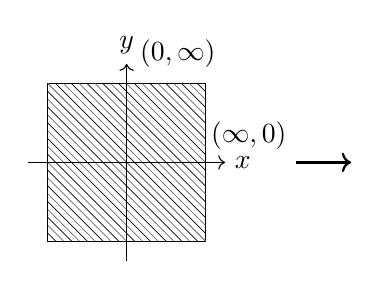
\begin{tikzpicture}
              \def\a{2}%width of rectangle
              \def\b{\a}%height of rectangle
              \def\lw{0.1}
              \draw[] (0,0) rectangle (\a,\b);
              \foreach \x in{0,0.2,0.4,...,\a}{
              \draw [gray,line width=\lw mm](\x,0)--(0,\x);
              \draw [gray,line width=\lw mm](\a,\x)--(\x,\b);}
              \foreach \x in{0.1,0.3,...,\a}{
              \draw [black,line width=\lw mm](\x,0)--(0,\x);
              \draw [black,line width=\lw mm](\a,\x)--(\x,\b);}
              \draw[->] (1,-0.25) -- (1,2.25cm) node[above] {$y$};
              \draw[->] (-0.25,1) -- (2.25cm,1) node[right] {$x$};
              \draw (2.55cm,1cm) node[above=1pt] {$(\infty,0)$};
              \draw (1.65cm,2.05cm) node[above=1pt] {$(0,\infty)$};
              \draw[->,thick]  (3.15cm,1) -- (3.85cm,1);
          \end{tikzpicture}
          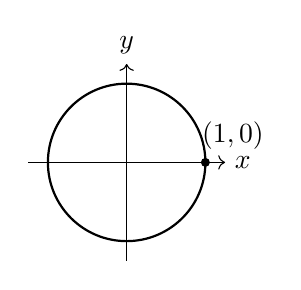
\begin{tikzpicture}
              \draw[thick] (0cm, 0cm) circle(1cm);
              \draw[->] (0,-1.25cm) -- (0,1.25cm) node[above] {$y$};
              \draw[->] (-1.25,0) -- (1.25cm,0) node[right] {$x$};
              \filldraw[black] (1cm, 0) circle(1.4pt);
              \draw (1.35cm,0cm) node[above=1pt] {$(1,0)$};
          \end{tikzpicture}
          \caption{Fix the optimized matrix eigenvalues onto the unit circle.}
      \end{figure}
    \end{frame}
  
    \begin{frame}{Summary}
      \begin{itemize}
        \item LSTM works like a differentiable memory chip.
        \item When in doubt, use LSTM.
      \end{itemize}
    \end{frame}

    \section{Applications}
    \begin{frame}{Language Processing}
      One hot encoding for letters. A possible encoding looks for all characters in a dataset.
      The number of occurring characters determines the length of every one-hot character vector.
      A system that accepts text and produces text, therefore, maps one-hot encoded sequences onto each other.
    \end{frame}


    \begin{frame}{Example: Machine Translation}
      \cite{Bahdanau2015NeuralMT} used RNN for the task of machine translation.
      \begin{figure}
      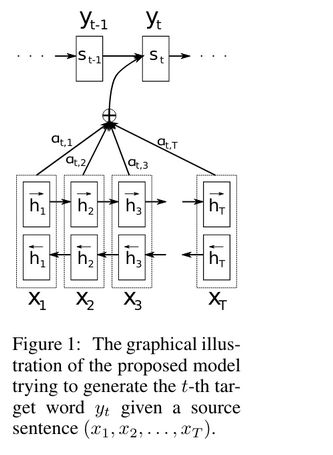
\includegraphics[scale=0.3]{./figures/translation.png}
      \caption{An RNN-based translation system. Figure from \cite{Bahdanau2015NeuralMT}.}
      \end{figure}
    \end{frame}

    \begin{frame}{Neural attention in machine translation}
      Attention weights group related inputs together,
      allowing a decoder to find a suitable translation.
      \begin{figure}
      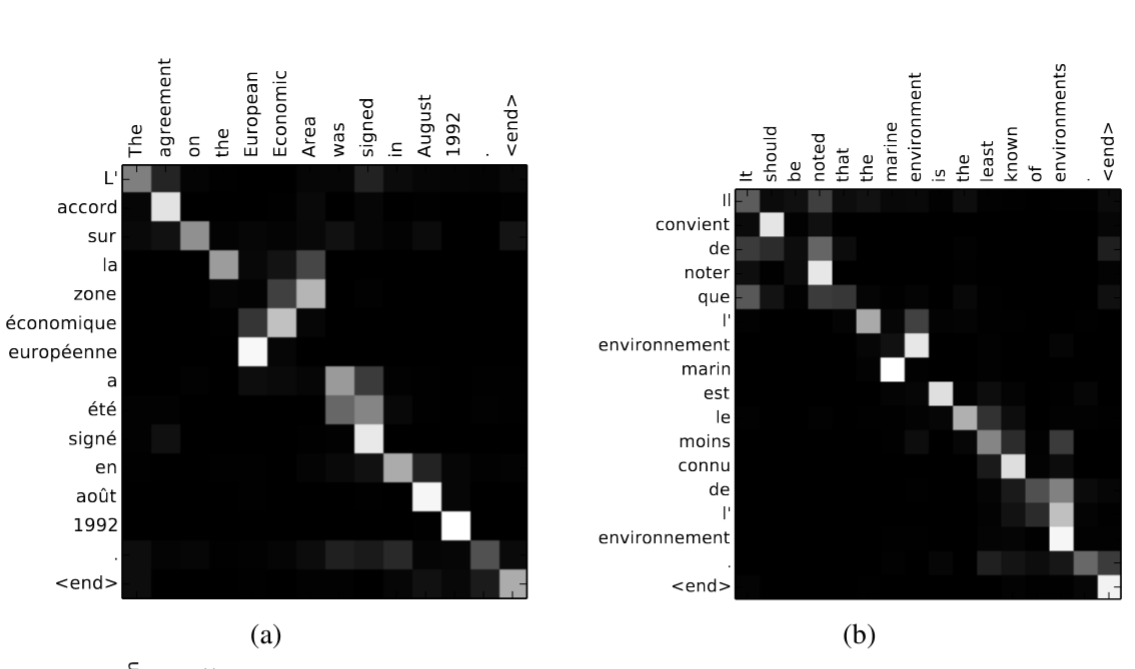
\includegraphics[scale=0.2]{./figures/attention.png}
      \caption{Attention plots as observed in \cite{Bahdanau2015NeuralMT}.}
      \end{figure}
    \end{frame}

    \begin{frame}{Neural Keyboard}
      Given a sequence of input letters or words LSTM, for example, can model
      the probability of the next letter or word.
      \begin{align}
        p_n(y_i| y_1, y_2, \dots , y_{i-1} = LSTM(y_{i-1}, c_{i-1}, h_{i-1})
      \end{align}
      This could, for example, help users type.
    \end{frame}

    \begin{frame}{Speech Processing \cite{chan2015listen}}
      \begin{figure}
        \includestandalone[width=.5\linewidth]{./figures/las_arc}
      \end{figure}
    \end{frame}

    \begin{frame}{Time-series forecasting}
        \begin{figure}
            \includestandalone[width=0.45\linewidth]{./figures/power_plot_intro}
            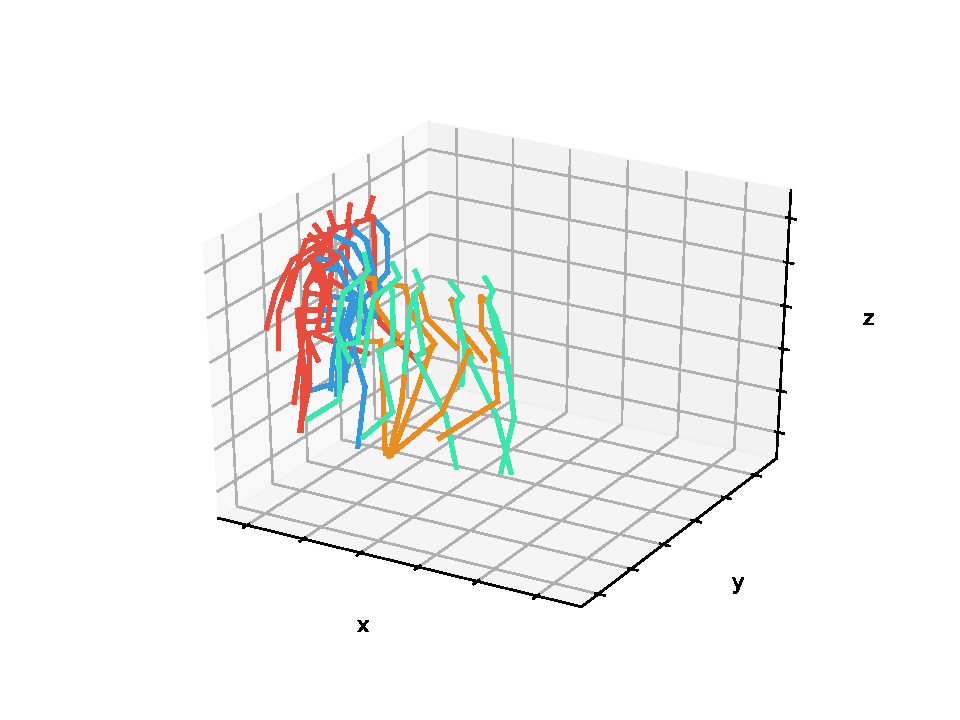
\includegraphics[width=0.5\linewidth]{./figures/test_figure17.pdf}
            \caption{Monovariate power-load and multivariate motion-capture time series data.}
        \end{figure}
    \note{
    Example time series data plots. \\
    Monovariate Belgian power load of January 2016. \\
    Task: Load prediction. \\
    Human3.6m walking motion sample. \\
    Task: Motion prediction for robots. }
    \end{frame}

    \begin{frame}{Day-ahead power-load}
        Day-ahead power load forecasting using European Network of Transmission system operators for electricity data: \cite{wolter2018fourieri}
        \begin{figure}
            \centering
            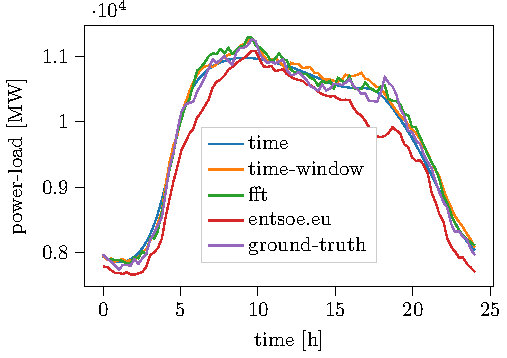
\includegraphics[width=0.49\linewidth]{./figures/day_ahead_plot.pdf}
            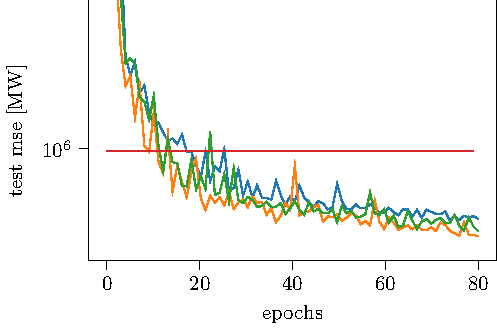
\includegraphics[width=0.49\linewidth]{./figures/power_pred_15min_1d_test.pdf}
        \end{figure}
        \note{Task: predict the power consumption on the next day at noon of the 
              previous day. \\
              Data: We use the power load data of 36 EU countries from 2011 to 2019 as provided by the European Network of Transmission System Operators for Electricity.
              We partition the data into two groups; thosereporting with a 15 minute frequency are used for day-ahead predictions, while those with hourly reports are usedfor longer-term predictions.
              For testing, we hold back the German Tennet load recordings from 2015, all of Belgiums recordings of 2016, Austrias load of 2017 and finally the consumption of the German Ampiron grid in 2018. \\
              Take away: All machine learning methods better than the official approach (unknown).
              }
    \end{frame}

    \begin{frame}{Mocap-Demo}
      \href{run:./figures/mocap_demo.gif}{Link to mocap demo}
    \end{frame}


    %\section{Attention and Transformers}
    %\begin{frame}{Attention}
    %  TODO
    %\end{frame}
    %\begin{frame}{Transformers}
    %  TODO
    %\end{frame}

    \begin{frame}{Conclusion}
      \begin{itemize}
        \item RNNs are versatile and suitable for many different sentence processing tasks.
        \item Let's explore a generative Language modeling example today.
      \end{itemize}
    \end{frame}

    \begin{frame}[allowframebreaks]{Literature}
      \printbibliography
    \end{frame}

    \subsection{Code snippets}
    \begin{frame}{Sequence coding with dictionaries}
      TODO
    \end{frame}

    \begin{frame}{Implementing an LSTM}
      TODo
    \end{frame}


    \subsection{Exercise: Play with generative Text models.}

\end{document}
